\chapter{Methodology}
\label{ch:method}

\begin{itemize}
\item explain that the dataset has a 3:1 split of cancelled to not cancelled
\end{itemize}

\section{...}
As previously mentioned, I am going to be using the CRISP-DM model (\cite{WirthCRISP-DM:Mining}) to break down the problem into 6 specific stages \textbf{reference the figure}.


\section{Business Understanding}

This sections asks the question of that exactly the business needs and hopes to gain from the process, in this case the business needs to gain a better understanding of which customers are most likely to cancel there bookings. Doing this will help to not only prevent bookings from being cancelled but also to gain a better overall understanding of why bookings are cancelled. 

\begin{figure}[hbt!]
 %\centering
 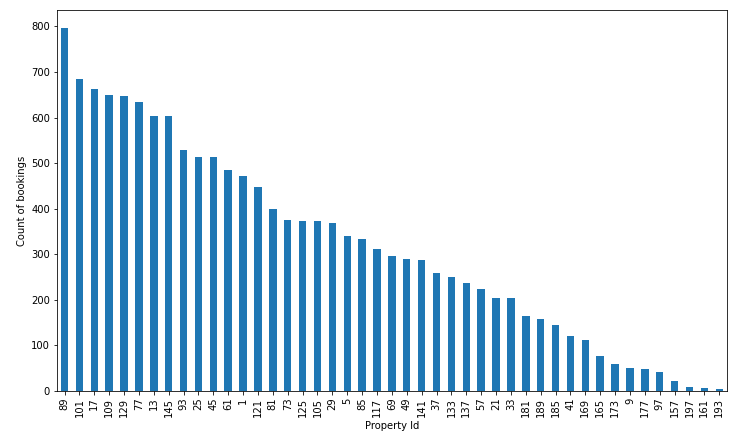
\includegraphics[width=10cm]{figures/bookings_by_property.png}
 \caption{The X axis shows each of the property Ids with the Y axis showing the total number of bookings made}
\end{figure}

In total the dataset contains 45 properties, for the purposes of this task I will be creating a combined model for all properties since there is not an adequate amount of data to create individual models on a property level. I will however be able to show predictions for each property. 

\begin{itemize}
\item cost benefit analysis 
\item potential gain \textbf{take this from intro}
\item talk about the technologies that will be used
\end{itemize}




\section{Data Understanding}
\textbf{
\begin{itemize}
\item include the total size of each property 
\item include lead time
\end{itemize}
}

\begin{itemize}
\item explain what a docker container is and how it is deployed in azure 
\end{itemize}


To get the relevant data for solving this problem I first had to approach the wider problem of developing a robust data warehouse [reference] I started by building a live and dynamic data stream that could take data from an external source and store it in the company data warehouse so I would be able to run new iterations of the model as new data came in. To facilitate the problem of having a dynamic data import stream I used the python object relation mapping library \cite{SQLAlchemyPython} since it has direct support for the python data library pandas []. Doing this allows me to read data in any supported format [supported formats] and store it in a SQL database with the correct data types. The data I need is stored in an Amazon S3 bucket, so I used the python S3 library Boto3 to read TSV files from blob storage every hour and stored them in the data warehouse. I then deployed this process onto a docker container.

The booking data relevant to this problem is created in an external system, this is the website front facing to the customers where each of the bookings are taken. As a booking is made through the website customer details are stored in the external website databases. This data includes personal information of the customer like name, address, date of birth and phone number. As the customer moves further through the booking process they are then taken to a page asking which university they will be attending and to make a selection of the property they want to rent. Here information like location of property, room name, price and extras are stored. When a student then selects a specific room they will be asked about the payment structure they want to use and how they will make there deposit. It is here that all of the relevant cost data is stored. \par

The information stored within these stages of the booking describes all of the intellectual property stored about each specific customer and therefore is what will be used to predict the activity of the customer and weather or not they will cancel there booking. 

In the case of a classification problem we can consider any attribute relevant if it influences the target variable. With the common goal in machine learning to obtain as much useful information as possible since [reference good number of data points for machine learning]

In this case I will be looking only at data from the years 2020 to 2021 since the old data is incomplete. During this booking cycle there are a total of around 16 thousand bookings  in some number of countries 

\begin{figure}[hbt!]
 %\centering
 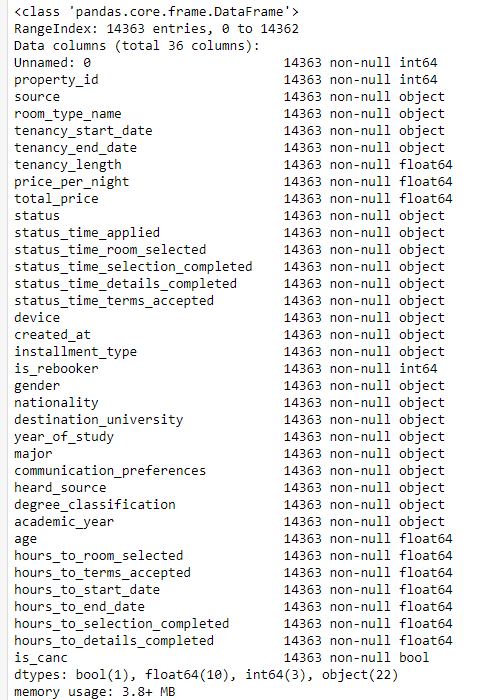
\includegraphics[width=10cm]{figures/df_info.png}
 \caption{}
\end{figure}

\begin{itemize}
    \item property id is the unique identifier for the residence 
    \item source is the internal system used to create the booking
    \item room type name is the category of room selected
    \item tenancy start date is the proposed start date of the contract
    \item tenancy end date is the proposed end date of the contract
    \item tenancy length is the duration in day the contract is valid for
    \item price per night is the daily rate at which the room will be sold
    \item total price is the total price for the contracted time
    \item status is the current status of the booking
    \item status time applied is the time the booking process was started
    \item status time room selected is the time the customer selected there room
    \item status time selection completed is the time the customer finalised the selected process 
    \item status time details completed is the time all personal details are entered
    \item status time terms accepted is the time the agreement is completed
    \item device is the type of the device the booking was made on
    \item created as is the time the process was started
    \item installment type is the payment schedule
    \item is rebooker defines if the same customer has applied before
    \item date of birth of the customer
    \item gender of the customer
    \item nationality of the customer
    \item destination university is the university the customer expects to go to
    \item year of study is the academic year  the customer is in
    \item major is the degree type of the student
    \item communication preference is the customer selected method of communication
    \item heard source is where the customer discovered the booking
    \item degree classification is the degree type of the customer
    \item academic year
 

\end{itemize}

 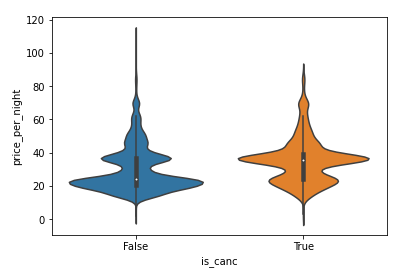
\includegraphics[width=10cm]{figures/price_per_night.png}
 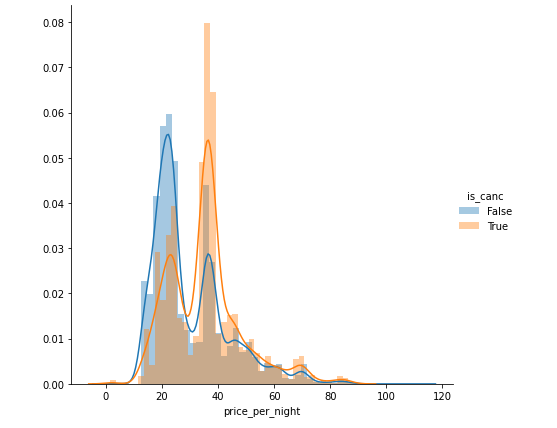
\includegraphics[width=10cm]{figures/price_per_night_2.png}
 
 looking at the price per night when comparing booking that canceled to ones that didn't we can see that around the middle price range of 40 euro per night is where the most significant number of bookings occur, the figure also shows more cancellations towards the higher end price points.  
 
 \textbf{how will this be used to help the model}
 
  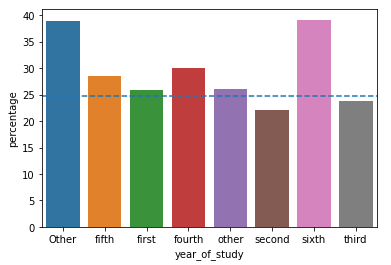
\includegraphics[width=10cm]{figures/canc_per_year.png}
  
  This figure shows a weighted proportion of customers canceling bookings in each year of study with the blue horizontal line being the average. We can see that sixth year students are more likely to cancel than any other year possibly because they are more likely to decide to live in private accommodation. The other category are students that didn't fill out the year of study section, this seems to be a good indication of cancellations.
  
  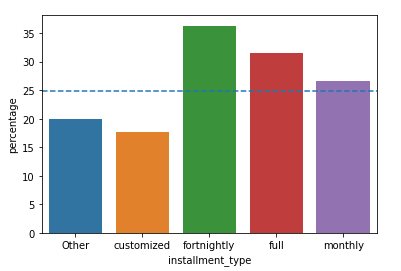
\includegraphics[width=10cm]{figures/instalment_type.png}
  
  This figure shows a weighted average of cancellations looking at the selected instalment type. Instalment type is the payment plan the student selected, we can see that students who selected the fortnightly plan are 10 percent more likely to cancel than the average and students who opted for the customized installment plan are around 6 percent less likely to cancel. this may be a good predictor of cancellations.
  
  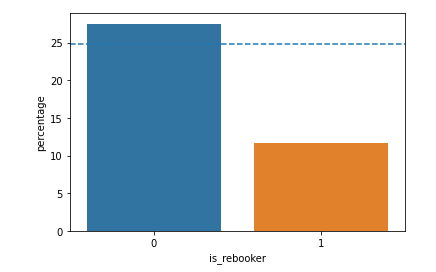
\includegraphics[width=10cm]{figures/is_rebooker.png}
  
  The figure above shows the comparison in cancellations with students who are rebookers (have booked before), we can see that students who have booked previously are around half as likely to cancel there bookings. this is another good predictor of cancellations.  
  

\section{Data Preparation}


With all of the necessary data stored in the data warehouse I imported the relevant tables into a Jupiter Notebook to preform the data cleaning stages. My aim is to include only valid bookings that made it the whole way through the booking process and then separate into cancelled or not.

I started by removing any booking in the dataset that didn't have a total price or with a total price less than 1 as this meant the booking was not stored in the system correctly and may have been used for testing. 

I then removed any booking that did not get to the terms accepted stage since this could not be treated as a cancellation or a booking as the customer process was not finished.

\begin{itemize}
\item include a screenshot of creating time features
\end{itemize}


Using the status time applied column to act as the first point where the booking process was started I created attributes used to store how long the customer took within each stage of the booking process as this may be able to indicate weather or not the user will cancel there booking.  \textbf{find a reference to support this}

\section{Modeling}

I used Azure ML Studio to evaluate and compare multiple different algorithms. ML studio is a cloud environment used to train, deploy, automate, manage and track ML models. It can be used for multiple different types of machine learning like supervised or unsupervised and deep learning. It gives the ability to write code in Python, R and its own no-code environment.  I used the cloud Jupiter notebook features for the data cleaning and preparation stages as well as testing models. To evaluate and compare multiple different algorithms I used the Automated ML feature on my cleaned dataset.

\begin{itemize}
\item splitting data into num and cat vars 
\item used SimpleImputer to replace missing num values with mean
\item train test split of 0.2
\item Azure ml - Azure machine learning studio [What is Azure Machine Learning | Microsoft Docs] is a cloud environment that can be used to both train and deploy machine learning models 
\item add some images of the azure ml stages
\item Azure Machine Learning SDK for Python
\item talk about how I run the results in python myself
\end{itemize}




\begin{itemize}
\item evaluation and deployment seem like part of the results
\end{itemize}

\section{Evaluation}

\section{Deployment}


